\chapter{Background}

This chapter is intended to provide information on some basic principles in terms of the Object Oriented Programming. The list is by no means exhaustive, however is meant to help understanding the focus of this thesis.

\section{Fundamentals of Object-Oriented Programming}

The paradigm of Object Oriented Programming (OOP) uses \emph{classes} as primary mean to gather and structure data. The data within a class is mostly called \emph{attributes}, means to interact with it are called \emph{methods} \cite[80]{Castagna97}. 

While a class is the abstract definition of such a container an \emph{object} is a concrete instance filled with actual data. Attributes that may differ between each instance are therefore also called \emph{instance variables}. Variables that belong to the class itself and thus are only instantiated once per class are called \emph{class variables}. 

\subsection{Encapsulation} 
To encourage refactoring \footnote{Refactoring describes the process of re-writing classes to improve readability, performance or other criteria while preserving its signature, inputs and outputs.} each class should prevent direct access to is internals from the outside. It should however provide a well-defined interface in terms of methods for manipulating the data, as this allows the class to enforce invariants \footnote{A invariant is some kind of requirement that must be fulfilled at all times before and after a method call. An example of such a invariant could be the descending sort order of an integer list.}. This means that it hides all information not relevant to others as they are only implementational details and thus not relevant. As other classes now rely on an interface rather than concrete implementations the code is called \emph{loosely coupled}. Modifying the internals now does not break interdependencies which encourages programmers to perform refactoring resulting in improved code quality. 

Many programming languages provide different access levels varying from visible to all others, accessible only within the class or visible from within and derived classes. The latter access level can be problematic as they effectively break the encapsulation. TODOTODO

\subsection{Inheritance}
Inheritance describes the concept of a child class inheriting all attributes, methods and other properties from a parent class. The child class is connected with the base trough a \emph{is-a}-relationship. The child is therefore a superset of the base class as it can be extended to meet the new requirements. This concept is important as it encourages developers to reuse existing code and in that way lower the risk of programming errors \cite{johnson91}. 

A prominent problem often mentioned in this context is the \emph{Diamond Problem} in the sense of multiple inheritance. It describes a situation in which at least two parents of a derived class share a single base class \cite{Truyen04}. If now a method of the topmost class is overridden by both ancestors of lowermost class, the question arises which of the two possible methods should be called. Some languages, such as Java or C\#, do not support multiple inheritance for this reason, while others explicitly allow it, such as C++ or Python. In this cases if a situation as described in the Diamond Problem arises the results can cause undefined behaviour.

\subsection{Polymorphism}

Polymorphism describes the ability to tie the same interface to different belonging types. TODOTODO citation There are two main kinds of polymorphism: The \emph{overriding} polymorphism, which is tied closely to inheritance and describes the ability to choose at runtime between equally-called methods and attributes of a base class and its child class. For example, if a base class \texttt{Animal} has a method \texttt{speak}, each derived class \texttt{Dog} and \texttt{Cat} both inherit this method. With overriding polymorphism if the method is called the two subclasses are able to behave in different ways while providing the same programming interface. It is determined at runtime which method should be executed for an object. 

The other important kind is \emph{overloading} polymorphism which is used to provide methods with the same name but different signatures (and thus attributes). An example could be two methods called \texttt{add}, one taking a number, one taking a text as a parameter. Here it is determined at compile time which method will be used. \footnote{https://docs.microsoft.com/en-us/dotnet/csharp/programming-guide/classes-and-structs/polymorphism, accessed 31.08.2017}.

\subsection{Single Responsibility Principle}
This important principle states that each class should only full-fill one particular purpose and as a result does only have one reason to change. The computer scientist D.L. Parnas wrote that in software development each design decision which is likely to change should be placed in a single, independent module and hides this decision from others \cite{srp}. When followed it avoids side effects on other responsibilities when changing the class. 

A example of a class violating this concept could be a class that reads two numbers from the user, calculates the sum and prints the result. While this program seems quite simple three different responsibilities are placed in the same class. If either the means to provide the input, for presenting need to be modified or the algorithms should support other data types, the class need to be changed. The modifications may introduce errors to the other functionality, which could be avoided if the program fould conform the principle. This would require placing each responsibility in a independent module.
\subsection{Open Closed Principle}
The Open-Closed-Principle states that each class should be open to extension and closed for modification \cite{ocp}. As already written code is assumed to be well tested and working as intended it should be avoided to modify it afterwards to add new functionality. Every change could lead to unwanted side effects that may only occur in very specific situations and are therefore difficult to detect. 

Inheritance addresses this problem as it empowers the programmer to add new features while preserving all of the old code. Even when overriding methods in terms of polymorphism the principle is not violated at the original class is preserved as-is. 

\section{Design Patterns and Architectural Patterns}
In opposite to the previous chapter which describes rather abstract guidelines in the object oriented programming this section focuses on widespread methods which try to help solving common problems that might occur in bigger projects. They are called \emph{design patterns} and are subject to a large amount of books, of which the most famous is probably \emph{Design Patterns - Elements of Reusable Object-Oriented Software} by Erich Gamma, Richard Helm, Ralph Johnson and Jphn Vlissides and \emph{Patterns of Enterprise Application Architecture} by Martin Fowler. While the former book is more focused on general programming patterns, the latter one is more relevant for bigger businesses where a multi-tier architecture (see section \ref{sec:multi-tier}) is more common. 

The main difference between architectural and design patterns lies in different phases they are applied at. Architectural patterns provide high-level strategies providing a big picture often describing the interaction between so-called \emph{components}, which can vary widely in its complexity and each of them providing a well-described service and fulfilling a certain purpose. Design patterns focuses more on the actual implementation and describes a way to solve a problem on class and interface level. 

\subsection{Repository}
\label{sec:repository}
The repository design pattern is a programming strategy that is useful when operating with some kind of data persistence service. It provides an abstraction layer between the business code and the place where data of the application is actually saved, providing a simple and clean interface for the business code and leads to a looser coupling. All actions dealing with specialized database operations, object retrieval and others are hidden by a repository, because of this it is considered part of a data-abstraction-layer (see section \ref{sec:multi-tier}). A repository is often used if only basic operations with the data source are necessary. Other patterns and frameworks supporting advanced functionality and are available however they are not relevant to this thesis.

To create one repository per business object (data class) is the most basic way of implementing this pattern. Asides from the basic \emph{CRUD}-Operations \footnote{Create, read, update, delete}, each repository should provide specialized object retrieval methods that are only valid for the business model it was programmed for. 

For example, in a booking system there may be a data class \texttt{Order}. A repository for this class may then provide a method called \texttt{getOrdersByUsername}. In general only methods that are actually needed should be implemented, which is described in the \emph{YAGNI}-principle \footnote{You aren't gonna need it}.


\subsection{Model-View-Controller}
The Model-View-Controller (MVC) is a pattern that describes a separation of a program in three layers, it is considered both a design and a architectural pattern, depending on the point of view.  Its goal is to improve flexibility and extensibility of an application which can help to improve maintainability. It consists of three components, from which the \emph{model} contains the business logic, the \emph{controller} processes interactions and the \emph{view} presents some kind of user interface. 

This pattern is not very well defined and is subject of constant discussions. While it is commonly agreed upon that the application should be split in the three layers, the data flows and connections between the components are described in many different ways. The original concept of MVC developed for Smalltalk as described before the model holds logic and data of the application. Views subscribe at the model for notifications on changes of data in order to be able to update and refresh themselves. The controller was responsible of managing user interaction, which includes switching between views and forwarding requests to the model. This situation can be seen in Figure \ref{fig:mvc-smalltalk}. This direct interaction between model and view is often not desirable, especially in the context of web applications, which leaves it deprecated today. 

\begin{figure}[htbp]
	\centering
	\label{fig:mvc-smalltalk}
	
	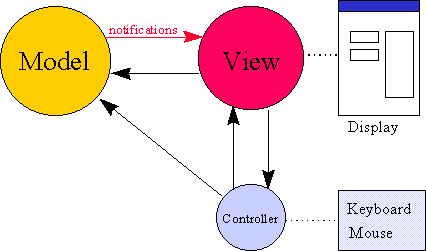
\includegraphics[width=0.5\textwidth]{./content/pictures/mvc-smalltalk.jpg}
	\caption{Classical Model-View-Controller concept as used in Smalltalk. Model and View know each other.}
	\caption*{Source: \href{https://www.mimuw.edu.pl/\~sl/teaching/00\_01/Delfin\_EC/Overviews/MVC.htm}{https://www.mimuw.edu.pl}, accessed 5.9.2017}
\end{figure}

\subsection{Model-View-Presenter}
The Model-View-Presenter (MVP) pattern is similar to the MVC-model as it shares the concept of separating the application into three layers. However the responsibilities differ considerably, as can be seen in Figure \ref{fig:mvp}. The view only communicates with the presenter and does not know about the model. The presenter handles user input and requests, gathers data from the model, updates it and finally is responsible for refreshing the view with new data. This implies that the model does not know about the existence of view or presenter and at least in the original concept of MVP all business logic is placed in the presenter classes. It is important to note that it is vital for the use of this pattern to implement it using interfaces. This ensures that its main goal, easy testability, can be reached easily. 

\begin{figure}[htbp]
	\centering
	\label{fig:mvp}
	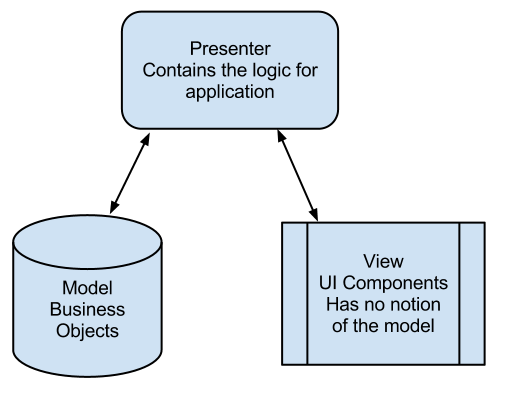
\includegraphics[width=0.5\textwidth]{./content/pictures/mvp.png}
	\caption{Diagram of Model-View-Presenter. While the view again only holds the means for displaying the data and interacting, in opposite to the MVC-model it does not know about the model but only corresponds with the presenter. The presenter is responsible for gathering the necessary data from the model and forwards it to the view. The model does not know about the presenter.}
	\caption*{Source: \href{https://de.wikipedia.org/wiki/Model-View-Presenter}{https://de.wikipedia.org/wiki/Model-View-Presenter}, accessed on 5.9.2017, by Daniel.Cardenas - Own Content, CC BY 3.0, https://commons.wikimedia.org/w/index.php?curid=19794348}
\end{figure}


After some years Martin Fowler drafted two design patterns that are closely connected to MVP. In his blog entry \footnote{\href{https://martinfowler.com/eaaDev/ModelViewPresenter.html}{https://martinfowler.com/eaaDev/ModelViewPresenter.html}} he explained that he felt the need to split the MVP-pattern into two resulting in the following concepts, briefly described in Figure \ref{fig:passive-view-supervision-controller}. 

\begin{figure}[htbp]
	\centering
	\label{fig:passive-view-supervision-controller}
	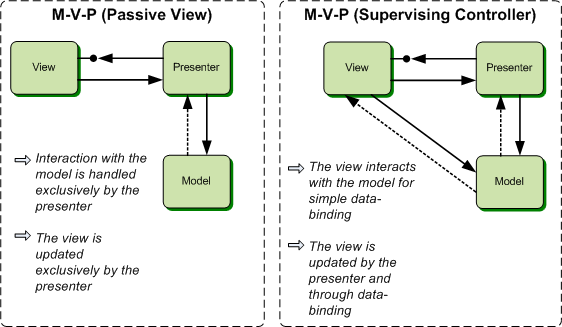
\includegraphics[width=0.5\textwidth]{./content/pictures/passive-view.png}
	\caption{Basic diagrams of the Passive View (left) and Supervising Controller patterns (right). In the former as little logic as possible is placed in the view making it easy replaceable by a mock object for testing. Synchronization logic needs to be placed in the Presenter. In the latter view and model are connected trough data bindings empowering these two to perform synchronization tasks on their own. This simplifies the role of the presenter.}
	\caption*{Source: \href{https://msdn.microsoft.com/en-us/library/ff709839.aspx}{https://msdn.microsoft.com/en-us/library/ff709839.aspx}, accessed on 5.9.2017}
\end{figure}

\subsubsection{Supervising Controller}
In this concept it is the views responsibility to perform data synchronization using shared classes between it and the model. This simplifies the tasks to be performed by the presentation layer while reducing the level of testability possible. 
\subsubsection{Passive view}
In the concept of passive view the model is not connected with the view, which in terms only corresponds with the presenter. It is desired to minimize the logic placed in the view, leaving it (as the name describes) passive and therefore easy to mock. This is especially useful for automated testing, as it allows the tester not only to test the basic logic placed in the presenter but also its synchronization capabilities. The drawback of this clearly lies in the additional responsibilities that need to be met by the presenter.

\footnote{http://www.wildcrest.com/Potel/Portfolio/mvp.pdf}


\subsection{Client-Server}
The Client-Server model describes a way to separate tasks within a network. While the client, which can be any kind of computer program, requests a resource from the server. It is designated to be used within the internet and is still on of the cornerstones of current web infrastructure. A prominent example of the client-server model is the Domain-Name-System (DNS). When a user types in the domain name of a service he wants to access, the browser needs to translate the name into a IP-Address he can work with. In order to do that he sends a request to a DNS-Server, making him a client. While he does not need to know how exactly the resolving takes places he requires the server response to have a certain format described in the communication protocol. 

There are several benefits of using this architecture. For starters it centralizes the administration which lowers the effort to managing access rights, accounts and so on. Because the important data is in one place it is easier to create backups and ensure security policies. However a server is considered a \emph{Single Point of Failure}, meaning that a whole service will be unavailable if the server for any reason is not reachable, making it a worthy target of attacks. While the impact depends on the actual service built, scalability and extensibility are important factors. It is easier to extend the features provided by a service when using the client-server-model it reduces scalability as the hardware needs to be upgraded from time to time to meet a increased number of requests directed to the server.
\begin{figure}[htbp]
	\centering
	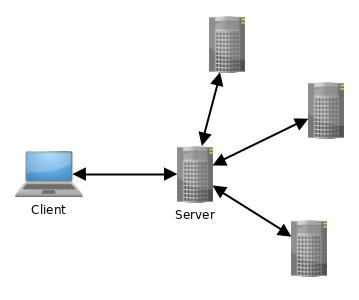
\includegraphics[width=0.5\textwidth]{./content/pictures/client-server.jpg}
	\caption{Client-Server setup. The client sends a request to a server by messages defined in the protocol. The processing of the request is transparent to the client, it does not know about the actions taken by the server and awaits a response in a certain format.}
	\caption*{Source: \href{https://abcnetworking.wikispaces.com/Client+Server+Networking}{https://abcnetworking.wikispaces.com/Client+Server+Networking}, accessed on 6.9.2017}
\end{figure}

\subsection{Peer-to-Peer}
Peer-to-Peer (P2P) infrastructure is the counterpart of client-server-models. No central server exists which means that each of the clients are equally featured, each client has the means to request and provide resources. P2P-Networks are considered more robust and scalable than Client-Server set-ups, as the failure of one node does not lead to the breakdown of the whole system.

\subsection{Multi-Tier and Multi-Layer Architecture}
\label{sec:multi-tier}
Multi-Tier architecture is mostly mentioned in the context of web applications. In general it describes the separation of responsibilities on different \emph{physical} places \footnote{In this context physical separation means that there has to be going on any kind of communication between independent processes within the same machine or connected trough the internet.}. This is the main difference to a multi-layer-system where the responsibilities are separated but placed at the same process which indicates the use of interfaces. 

A 3-Tier-Architecture nowadays refers mostly to the typical set-up of a web application as it can be seen in Figure \ref{fig:multi-tier}. It has to be noted that it is very common to use multi-tier and multi-layer architecture mutually. For example, the logic tier in the figure could use a data-access-layer to abstract the communication with the data tier. 

\begin{figure}[htbp]
	\centering
	\label{fig:multi-tier}
	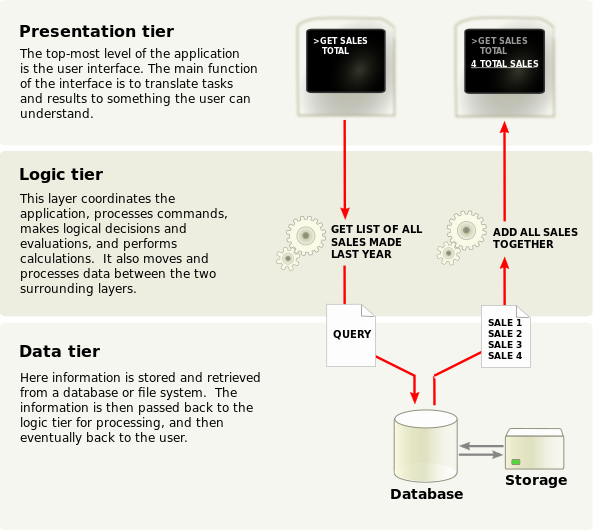
\includegraphics[width=0.5\textwidth]{./content/pictures/multi-tier.jpg}
	\caption{Multi-Tier set-up. The tiers are physically separated.}
	\caption*{Source: \href{https://en.wikipedia.org/wiki/Multitier\_architecture}{https://en.wikipedia.org/wiki/Multitier\_architecture}, accessed on 6.9.2017}
\end{figure}

\section{Technologies}
\subsection{Java}
This project is written in Java, an object oriented programming language released by Sun Microsystems in 1995  \footnote{\href{https://java.com/en/download/faq/whatis_java.xml}{https://java.com/en/download/faq/whatis\_java.xml}, accessed 7.9.2017}. In 2010 the company Oracle bought it and is developing and distributing the language since. It is split up into two main components, its development kit (JDK) and its runtime environment (JRE). The JRE is providing a virtual environment called Java Virtual Machine (JVM) which is used to run so-called Java Bytecode which is comparable to x86 assembler. This bytecode can be compiled from plain Java programs as well as other languages such as Scala or Groovy. 
This approach helps reaching one major goal of the language: portability. Java bytecode can be executed on every platform, as long as a JRE is installed, which nowadays includes mobile phones, embedded platforms and with reduced functionality even smart cards \footnote{\href{http://www.oracle.com/technetwork/java/embedded/javacard/overview/index.html}{http://www.oracle.com/technetwork/java/embedded/javacard/overview/index.html}, accessed 7.9.2017}. 

The JRE uses an interpreter and a just-in-time (JIT) compiler to generate native machine code that can be executed of the platforms processor. A JIT-Compiler generates the necessary machine code at runtime for some parts of the application. This can lead to significant performance improvements compared to the exclusive use of an interpreter.

As of September 2017 according to the TIOBE-Index it is the most popular programming language with a share of more than 12\% \footnote{\href{https://www.tiobe.com/tiobe-index/}{https://www.tiobe.com/tiobe-index/}, accessed 7.9.2017}. 
\subsection{Swing}

Swing is a Graphical-User-Interface (GUI) Library for Java and was first published in 1997. It is rendered directly by Java thus it is not necessary for a platform to provide specific controls. However this leads to a significant difference to applications natively written for the platform as some control concepts may differ or buttons may be placed at other positions. This problem is bypassed by the introduction of different \emph{Look-and-Feels} which intend to adopt the application to be as similar to a native program as possible.

\subsection{JavaFX}

JavaFX is a framework \footnote{The main difference between a framework and a library is the so-called \emph{Inversion of Control}. While a library is called by the programmer, when using a framework it is in control and calls methods provided by the developer.} for GUI programming in Java and was released in 2014, replacing Swing as the main method for graphical programming. In opposite to Swing it implements its own multimedia-stack able to access graphics card feature through OpenGL and Windows Direct3D.  

\subsection{Relational Databases and PostgreSQL}

PostgreSQL is a open source object-relational database management system (ORDBMS) that was first published in 2002. Other than many database management systems it is focused on maintaining a good SQL standard compliance and is currently ranked as the 4th most popular engine. \footnote{ \href{https://www.postgresql.org/about/}{https://www.postgresql.org/about/}} \footnote{\href{https://db-engines.com/de/ranking}{https://db-engines.com/de/ranking}}

Almost all database systems that are considered as relational use the Structured Query Language (SQL) or a dialect of it as language for querying and manipulating the database. Such a system is characterized by structuring the data into \emph{tables}, which consists of \emph{columns} and \emph{rows} (also: \emph{records}). Many systems require each row to have a unique identifier, also called \emph{primary key}. This key can consist of one or more columns per row, if more columns are considered it is also called \emph{composite key}. 

If it is wanted to refer from one table row to the a record from another table a \emph{foreign key} is used which corresponds to the primary key of the original table. This is vital for maintaining the so-called \emph{referential integrity}, which indicates that all references have valid targets. Depending on the policy set in the database management system or specified in the foreign key definition of the table the deletion of a row that is referred by another record could be prevented.


\subsection{MongoDB}
As a prominent example for NoSQL\footnote{Not only SQL}-databases MongoDB is a database engine written in C++ and published in 2009. In opposite to relational databases it persists the data in \emph{documents} which are structured in a JSON\footnote{JavaScript Object Notation, a syntax for exchanging data which is easy to read for humans and efficiently processable by machines. It is build around key-value-pairs which can be nested.}-like manner. 

Documents can be stored in \emph{collections} which are comparable to tables in SQL-databases. While all rows in tables possess the same columns this is not necessarily true for collections. Each document in a collection can hold arbitrary attributes which improves the flexibility while as a trade-off reducing data integrity. In opposite to relational databases in MongoDB foreign keys cannot be created, however each document is provided with a built-in unique identifier.

\subsection{Caching}

Caching is the process to hold often needed data in memory to reduce the time necessary for gathering. While most of modern database management systems already provide advanced caching techniques out of the box, the application could be physically separated from the server by a low-bandwidth network. Therefore client-side caching may be necessary for reducing latency. 

In most of the cases placing the cache in the data access layer (see section \ref{sec:multi-tier}) leads to the simplest implementation as all data accesses are passing through here, however depending on the structure and needs of the application it may be necessary to implement the cache in the business code.

\subsubsection{Caching strategies}
There are two main types of caching policies: \emph{write-through} and \emph{write-back}. When performing write-trough-caching all data is first persisted and then immediately updated in the cache, this operation blocks until all necessary writes are completed. This ensures that at all times a up-to-date copy of the data is available \footnote{\href{http://searchsolidstatestorage.techtarget.com/answer/Comparing-write-through-write-back-and-write-around-caching}, accessed 10.9.2017}. 

The write-back-policy on the other hand also caches write accesses without directly persisting it. The write operation onto the data tier is being performed asynchronously, this may then happen when the system load is low and therefore the overall performance may be improved. However it is considered more dangerous in terms of data loss due to system crashes or other errors as the only valid copy of the data is only resided in the cache  \footnote{\href{http://www.computerweekly.com/feature/Write-through-write-around-write-back-Cache-explained}{http://www.computerweekly.com/feature/Write-through-write-around-write-back-Cache-explained}, accessed 10.9.2017}.

\subsubsection{Cache Replacement Policies}
As memory is a scare resource it is necessary to limit caching space and thus not all data can be cached at the same time. This introduces the necessary of means to decide which cache entries are to abolish, this mechanism is called a \emph{Cache Replacement Policy}. 

The best policy clearly would be to replace the cache entry that will be needed again the latest. This is information that is not available the associated \textbf{Bélády's algorithm} is considered theoretical and is only used for measuring and comparing the performance of other policies.

There are several possibilities which differ significantly depending on the data access pattern (list not exhaustive):
\begin{itemize}
	\item \textbf{First-In, First-Out (FIFO)}: When caching with the FIFO policy as soon the cache runs full the \emph{oldest} entry will be replaced. This is typically implemented as a Queue because it reduces the efforts to keep track of the entries age.
	\item \textbf{Least Recently Used (LRU)}: This algorithm keeps track of the last reference to cache entries. When a replacement is necessary it frees the page which reference dates back the longest. 
	\item \textbf{Least Frequently Used (LFU)}: Research has shown that LRU performs poorly for some access patterns, so instead of deciding which page is to replace upon the access time, LFU decides upon the number of accesses.
	\item \textbf{Most Recently Used (MRU)}: Access patterns exist where it is preferred to abolish the entry that was accessed most recently, an example for this scenario would be the sequentially scanning of a file. The implementation is very similar to LRU.
	\item \textbf{Random}: Interestingly research has shown that random replacement can be considered a good strategy as well, especially as it is easy to implement and efficient. Most of the more advanced policies may perform better with certain access patterns while performing worse in others. In many cases it is not possible to predict how the accesses will take place which introduces the risk of experiencing a unfavourable pattern. Random replacement is not sensitive to this problems while providing solid performance.
\end{itemize}

\subsubsection{Cache invalidation}
In the context of cache invalidation a quote from Phil Karlton is especially famous\footnote{It is not clear if the quote is genuinely made by Karlton, however it is generally attributed to him.}: 
\begin{quote}
There are only two hard things in Computer Science: cache invalidation and naming things.
\end{quote}

A Cache invalidation mechanism is necessary if the data tier can be updated from more than one location or clients which is especially in the terms of web application the standard case. 

Most caching strategies therefore feature a so-called time based expiry. It provides each cache record with a time-out after that it will be evicted \footnote{\href{http://tutorials.jenkov.com/software-architecture/caching-techniques.html}{http://tutorials.jenkov.com/software-architecture/caching-techniques.html}, accessed 10.9.2017}

Another method is active cache invalidation which evicts either cache entry or the whole cache after a change in the data tier. To support this some kind of messaging mechanism is necessary to let the persistent storage notify all clients about the update. 

In the case of multiple clients it has to be noted that it could be desirable to store additional version information for the table rows, for instance a incrementing counter or a hash of the data set. Because of the possibility of multiple clients updating the same row concurrently from different locations race conditions can occur that lead to the overwriting of newly entered data. Even with active cache invalidation it cannot be guaranteed that the update notification reaches the second client in-time. 